% vim: ft=tex
\documentclass[11pt, a4paper, USenglish]{article} % change ``USenglish'' to ``norsk'' if applicable.

% Search http://ctan.org or type texdoc <package name> in a terminal to access LaTeX package documentation.
\usepackage{babel} % babel and csquotes are packages for multilingual (e.g. Norwegian) support.
\usepackage[T1]{fontenc} % See http://tex.stackexchange.com/questions/664/why-should-i-use-usepackaget1fontenc
\usepackage[utf8]{inputenc} % See http://tex.stackexchange.com/questions/44694/fontenc-vs-inputenc
\usepackage{csquotes} % Needs to be loaded after inputenc.
\usepackage{amsmath} % See: http://tex.stackexchange.com/questions/32100/what-does-each-ams-package-do
\usepackage{amssymb} % See above.
\usepackage{graphicx} % Provides the \includegraphics command.
\usepackage{listings} % Provides source code listings.
\usepackage{cleveref} % Provides the \Cref command, for cross-referencing of equations, sections, figures and tables.
\usepackage{todonotes} % Provides several handy TODO commands.
\usepackage[backend=biber, style=numeric]{biblatex} % http://tex.stackexchange.com/questions/25701/bibtex-vs-biber-and-biblatex-vs-natbib
\usepackage{hyperref} % Provides clickable links. Always load last.

\addbibresource{bibliography.bib} % Makes the bibliography file available to biblatex.

% ``listings'' package settings
\definecolor{dkgreen}{rgb}{0,0.6,0}
\definecolor{gray}{rgb}{0.5,0.5,0.5}
\definecolor{pink}{rgb}{0.63, 0.13, 0.94}
\lstset{language=Matlab, 
	keywords={break, case, catch, continue,else,elseif,end,for,function,
		global,if,otherwise,persistent,return,switch,try,while},
	basicstyle=\ttfamily,
	keywordstyle=\color{blue},
	commentstyle=\color{dkgreen},
	stringstyle=\color{pink},
	numbers=left,
	numberstyle=\tiny\color{gray},
	stepnumber=1,
	numbersep=10pt,
	backgroundcolor=\color{white},
	tabsize=4,
	showspaces=false,
        showstringspaces=false}


\title{ITK LaTeX Lab Report Template}
\author{Group XX\\789456 \\789457 }
\date{January 1, 1970}

\begin{document}
\begin{titlepage}
    \maketitle
    \begin{figure}
    \centering
    
\includegraphics[width=0.5\textwidth]{figures/logontnu_eng}
    \end{figure}
    \thispagestyle{empty}
\end{titlepage}
 
% \input vs. \include http://tex.stackexchange.com/questions/246/when-should-i-use-input-vs-include
% The short story is that \include forces page breaks while \input simply inserts the contents of the file.

\newpage
\begin{abstract} 
%\addcontentsline{toc}{section}{Abstract} % add this if you want the abstract in the table of contents.
This document outlines a few important aspects of the lab report. It contains some advice on both content and layout. The \LaTeX{} source for this document is also published, and you can use it as a template of sorts for your own report.

When you write your own report, this section (the abstract) should contain a \emph{very} short summary of what the lab is about and what you have done.
\end{abstract}

\thispagestyle{empty} % Avoid page numbering on the abstract page.

\newpage
\tableofcontents
\thispagestyle{empty} % Avoid page numbering on the table of contents.

\newpage
\setcounter{page}{1}
% vim: ft=tex
\section{Introduction}
Your introduction should contain an overview of the work you were assigned, as well as a few sentences putting the work into a larger perspective. You should also give a quick description of how the report is organized (as is done below).

You should of course put most of the work into doing good work in the lab and then presenting it in the report. When presenting your work in the report, both content and presentation/layout matters. Since your only way of communicating your good effort in the lab is through writing about it here, the way you write about it is essential. This means that even if you have the very best controller but describe it poorly, you will probably not be rewarded for the good results. A plot showing perfect control is worth very little if it is not accompanied by a clear description of what it represents.

Layout is naturally less important than content, but it still matters. You can think of report writing like selling an apartment; when you present your apartment for potential buyers you will of course clean the apartment and make it good looking. How clean the apartment is does of course not determine its value, but it is still important since it influences the subjective value your buyers will put on the apartment. 

\subsection{Software}
You are of course free to use whatever software you want for report writing. You can also submit a handwritten report, although this is probably not a great idea if your handwriting can be hard to read. 

You can also use Word or a similar word processor. However, it is next to impossible to achieve decent layout with Word. The support for vector graphics (discussed later) is extremely poor, and text tends to look pretty bad (bad support for kerning and ligatures). Furthermore, math is both time consuming and difficult to input, and tends to look very ugly. In general, a report written in Word looks like a draft.

It is strongly recommended to use Latex. Unless you tweak the layout too much, your report will almost certainly look very good. Although it can take a bit of effort to get started, it is also much quicker to use than Word and similar programs. The support for math and vector graphics is also great.

If you are new to Latex, you can have a look at the source for this document to get started. You can also look at the presentation by \cite{Berland2010} (in Norwegian) or consult \cite{Oetiker2011}. Another good reason to learn Latex is that you probably don't want to write your master's thesis in something like Word, doing so would likely be very frustrating. Being reasonably fluent in Latex before you get that far will make your thesis work much smoother.

Some of you are probably fluent in Latex and might plan to write the report using it. Please resist the temptation (if any) to change the fonts, make super fancy headers (they are not necessary for a report like this), change the margins, change the paragraph indentation and/or spacing, and similar things.

A great tool for collaborating on Latex documents is ShareLaTeX at \url{https://www.sharelatex.com/}; if you use this you won't have to install anything on your computer. Texmaker at \url{http://www.xm1math.net/texmaker/} is a good cross-platform editor. Some people like Lyx, which is a Latex editor that behaves a little bit like Word. If you prefer to compile your Latex document on the command line, the latexmk \url{https://www.ctan.org/pkg/latexmk} command is a great tool included in most TeX distributions. There is also a simple Vim plugin that uses latexmk as its backend called LaTeX-BoX \url{https://github.com/LaTeX-Box-Team/LaTeX-Box}.

\subsection{Other Comments}
If you have problems with Latex, the solution is usually just a few Google searches away.

You can write the report in Norwegian or English. Writing in English is encouraged and is great practice, but entirely optional. \emph{Do not interpret any of the advice or suggestions here as requirements.}

This report is organized as follows: Section~\ref{sec:prob_descr} contains some equations relevant for TTK4135, and some tips on how to create illustrations. Several \LaTeX{} tips can be foundin Section~\ref{sec:latex_tips}, such as how to create a table and matrix equations. Section~\ref{sec:figures} contains some advice on using plots from MATLAB\@. The closing discussion and concluding remarks are in Sections~\ref{sec:discussion} and~\ref{sec:conclusion}, respectively. Appendix~\ref{sec:matlab} contains a MATLAB file while Appendix~\ref{sec:simulink} shows an example Simulink diagram. The Bibliography can be found at the end, on page~\pageref{sec:bibliography}.

\section{Useful hints}
\subsection{The \texttt{\textbackslash input\{\}} command}
By using \texttt{\textbackslash input\{whatever\}} in your main tex file (\texttt{main.tex} in this case), the content of \texttt{whatever.tex} will be included in your pdf. This way you can split the contents into different files, e.g. one for each problem of the assignment. This makes it easier to restructure the document, and arguably improves the readability of the tex files. For instance; maybe you want each problem to start on a new page? Simply add \textbackslash newpage before each \texttt{\textbackslash input} command.

\subsection{Citations}
In academic writing, it is important to credit your sources. In \LaTeX this is done by the \texttt{\textbackslash cite} command. For instance \texttt{\textbackslash cite\{chen2014linear\}} will produce \cite{chen2014linear}, and make the full details of that source available in the references. This requires that you make a bibliography file (\texttt{ref.bib} in this case), containing something like
\lstinputlisting[language=Tex, firstline=1, lastline=10]{ref.bib}

There are many different citation styles, and a lot of customization that is possible, so please check out e.g. \cite{wikibookLatex}\footnote{Even though this cites a web page, scientific writing tries to keep the citation of web pages to a minimum.}.

% vim: ft=tex
\section{Useful packages}
This section lists some packages that are useful for reports. See also the comments in the preamble of this document.

\begin{description}
  \item[amsmath] provides some useful mathematical definitions (like \texttt{\textbackslash{sin}} for e.g. $\sin(\omega t)$ and \texttt{\textbackslash{lim}} for e.g. $\lim_{t\to\infty}$. Also some definitions to make it more convenient to write the math.
  \item[amssymb] provides an extended symbol collection.
  \item[hyperref] makes it possible to create ``clickable'' links, like \url{itk.ntnu.no/fag/TTK4115}, but also \cref{tab:extab}, \cref{eq:mmot} and \cref{eq:mmot2}.
  \item[graphicx] provides some useful definitions for dealing with graphics, like \textbackslash{textwidth}: \textbackslash{includegraphics}[width=\textbackslash{textwidth}]\{picture\} will have the same width as the text column.
  \item[float] lets you force placement of floats with the [H] option. You should normally not need this.
\end{description}
\begin{table}
  \caption{Example table}
  \centering
  \begin{tabular}{ll}
    \hline
    \textbf{X} & \textbf{Y}\\
    \hline
    5 & 8\\
    6 & 9\\
    7 & 10 \\
    \hline
  \end{tabular}
  \label{tab:extab}
\end{table}

\begin{subequations}
  \begin{align}
    J_p\ddot{p} &= L_{1}V_{d} \label{eq:mmot1}\\
    J_e\ddot{e} &= L_{2} \cos(e) + L_3 V_s \cos(p) \label{eq:mmot2}\\
    J_\lambda \ddot{\lambda} &= L_4 V_s \cos(e) \sin(p) \label{eq:mmot3}
  \end{align}
  \label{eq:mmot}
\end{subequations}

More information on these packages can be found in the documentation for each package. The following subsections include some other packages that require a more in-depth explaination.

\subsection{listings}
The \texttt{listings} package makes it easy to include code in the report. For example \cref{lst:label} includes code that is written in the tex file. However \cref{lst:listing2} simply takes the code directly from the source file. You can also specify what the code listings should look like: color, line numbers, frames\ldots

\begin{lstlisting}[caption={Some Matlab code, with the source in the tex file},label={lst:label},language=Matlab, float]
  degree = 6;
  out = ones(size(X1(:,1)));
  for i = 1:degree
  for j = 0:i
  out(:, end+1) = (X1.^(i-j)).*(X2.^j);
  end
  end
\end{lstlisting}
\lstinputlisting[language=Matlab, firstline=4, lastline=10, caption={Another piece of code, directly from the source file}, label={lst:listing2},float]{some_function.m}
This is great! However, try to keep the amount of code in the report to a reasonable level, and remember; code in itself is not an explanation.

See \url{http://ctan.mirrors.hoobly.com/macros/latex/contrib/listings/listings.pdf} for more information.

\subsection{todonotes}
The \texttt{todonotes} package is great for work in progress. Few things are more embarrassing than forgetting to remove ``LALALALAL FIXME!!!!!!'' from the middle of your report. Instead, use \texttt{\textbackslash{todo}\{LALALA FIXME!!!\}} \todo{LALALA FIXME!!!}. This will show up like a red box in the margin. Some prefer \texttt{\textbackslash{todo}{[inline]}\{FIXME2!!!\}} which produces \todo[inline]{FIXME2!!!} To avoid typing [inline] all the time, you can define
\begin{lstlisting}[language=TeX, numbers=none]
  \newcommand{\TODO}[1]{\todo[inline]{#1}}
\end{lstlisting}
in the preamble of the document, and then use \textbackslash{TODO}.

And the best part: When you are finished with your report (or have run out of time) you can simply change \textbackslash{usepackage}\{todonotes\} to \textbackslash{usepackage}[disable]\{todonotes\} and they will all magically disappear!

You can also use \textbackslash{listoftodos} to get a list of all the todos in your document, and \textbackslash{missingfigure} will create a dummy figure, like \cref{fig:my_awesome_fig}, that you can replace once you have made a proper figure. This way you can start referencing figures/plots before you make them, and still be reminded that you need to make them.

See \url{http://ctan.math.utah.edu/ctan/tex-archive/macros/latex/contrib/todonotes/todonotes.pdf} for more information.
\begin{figure}[h]
  \centering
  \missingfigure{Drawing of such and such}
  \caption{Sweet figure, bro!}
  \label{fig:my_awesome_fig}
\end{figure}

\subsection{cleveref}
Speaking of referencing: The observant reader might have noticed the use of \texttt{\textbackslash{cref}} in referencing tables, figures etc. This is a bit more clever than the normal \texttt{\textbackslash{ref}} because it detects what you are referencing based on the prefix of the label. Then it prints the appropriate ``prefix''. So \texttt{\textbackslash{cref}\{fig:my\_awesome\_fig\}} will produce \cref{fig:my_awesome_fig}, whereas \texttt{\textbackslash{cref}\{tab:extab\}} will produce \cref{tab:extab}. Notice how the labels of the table and the figureare prefixed with \texttt{tab:} and \texttt{fig:} respectively. If you want it to say e.g. ``figure'' instead of ``fig.'', this is completely customizable. There is also \texttt{\textbackslash{Cref}} for a capitalized version.

See \url{http://mirrors.ibiblio.org/CTAN/macros/latex/contrib/cleveref/cleveref.pdf} for more information.

\section{Summary}
Hopefully this has been a useful short guide. Please also check out the tex source code. For more inspiration check out \cite{wikibookLatex}. Also, since \LaTeX is so extensively used, StackExchange and Google generally has the answers you are looking for.


\newpage
\addcontentsline{toc}{section}{Appendix} % comment out this if you don't want the appendix included in the table of contents.
\appendix
\section{MATLAB Code}\label{sec:matlab}
This section should contain your MATLAB code. DO NOT attach files posted online (that you didn't write). Note that the method used to input code below does not look as pretty when the lines are too long.

\subsection{plot\_constraint.m}\label{sec:plot_constraint_m}
\lstinputlisting{code/plot_constraint.m}
\section{Simulink Diagrams}\label{sec:simulink}
This section should contain your Simulink diagrams. Just like the plots, these should be in vector format, like in Figure~\ref{fig:simulink}. Make them tidy enough to understand.

\subsection{A Simulink Diagram}
Figure~\ref{fig:simulink} shows a Simulink diagram.
\begin{figure}[htb]
	\centering
		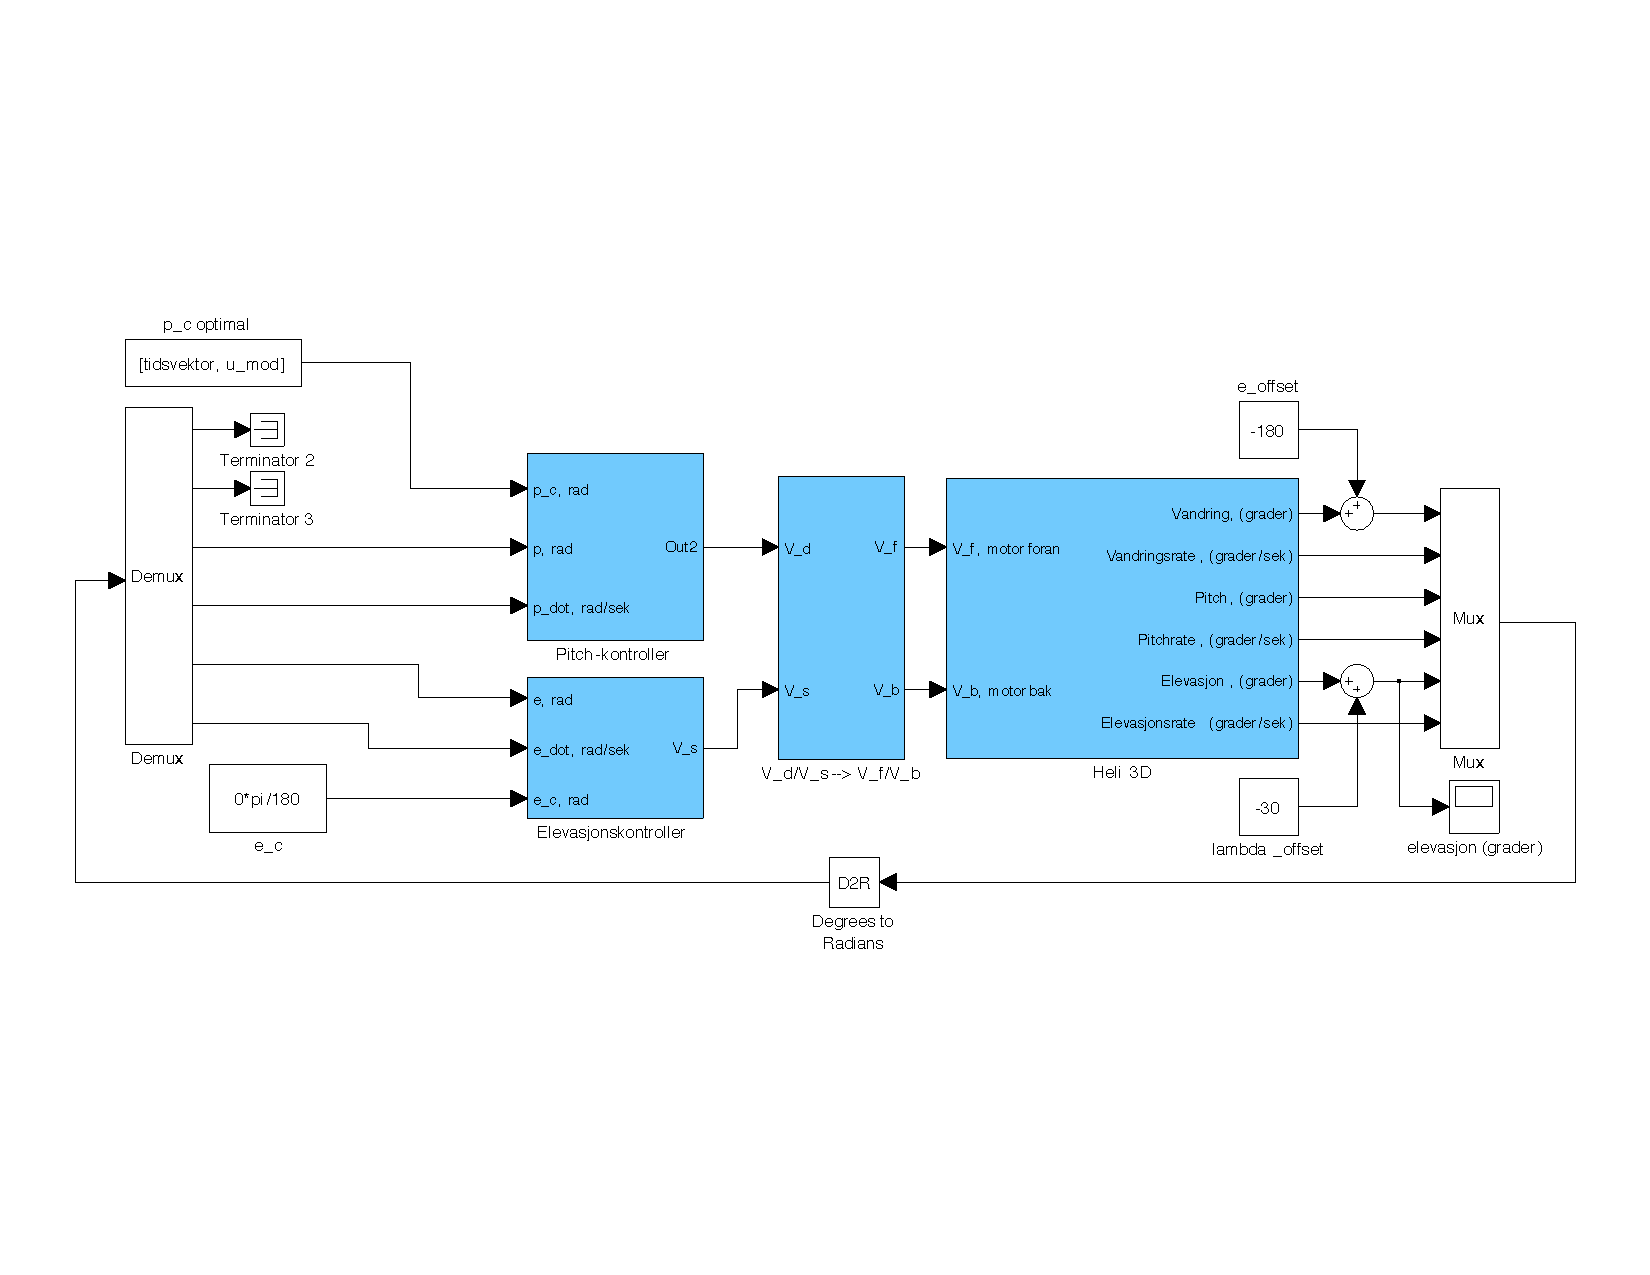
\includegraphics[width = \textwidth]{figures/simulink.pdf}
	\caption{A Simulink diagram.}
	\label{fig:simulink}
\end{figure}

\newpage
\addcontentsline{toc}{section}{References}
\printbibliography

\end{document}
